\chapter{RV12 Execution Pipeline}

The RV12 implements a 32/64bit Integer modified form of the classic RISC pipeline.
The pipeline consists of the Instruction Fetch, Pre-Decode, Instruction Decode, Execution, Memory Access, and Write Back stages as highlighted in the figure below.


\begin{figure}[!htb]
  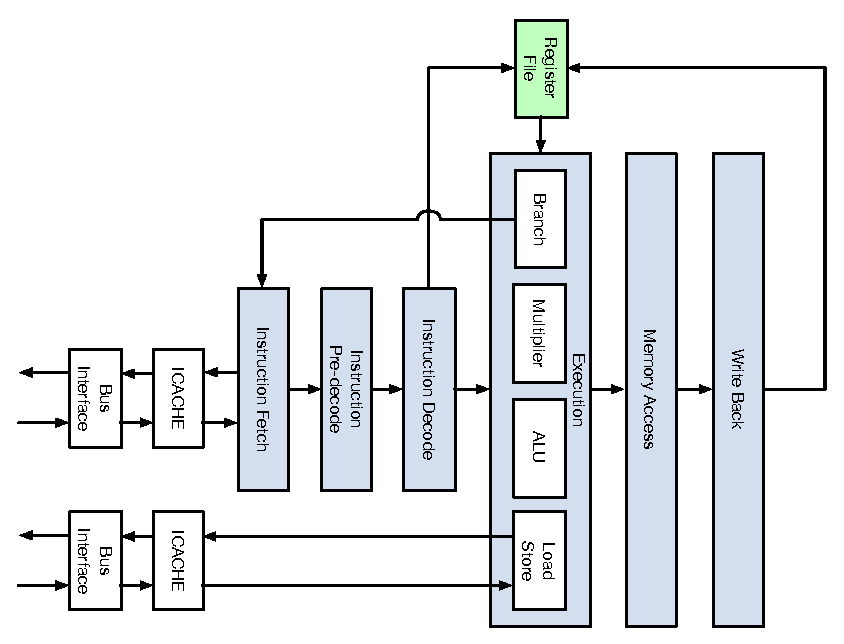
\includegraphics{assets/img/Pipeline-Overview}
  \caption{RV12 Execution Pipeline}
\end{figure}

\pagebreak

\section{Instruction Fetch (IF)}\label{instr-fetch-if}

The Instruction Fetch unit loads a new parcel from the program memory.
A parcel is a code field that contains one or more instructions.
The address of the parcel to load is held by the Program Counter (PC).
The Program Counter is either 32 or 64bits wide, depending on the XLEN parameter.
The Program Counter is updated whenever the Instruction Pipeline is not stalled.

If the pipeline is flushed the Program Counter is restarted from the given address.

\begin{figure}[h]
  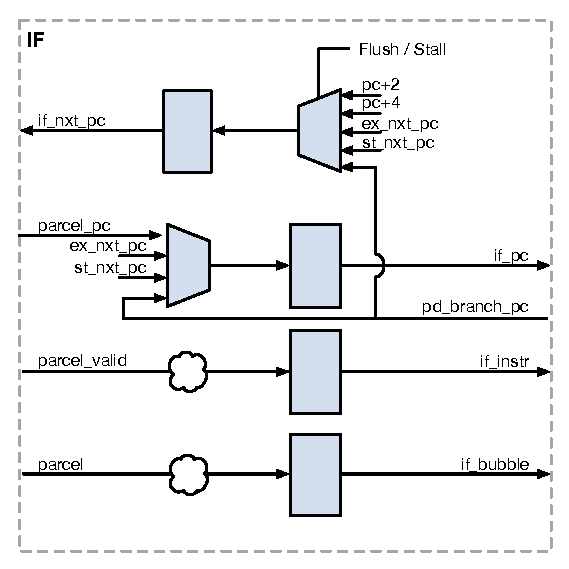
\includegraphics{assets/img/Pipeline-IF}
  \caption{Instruction Fetch Stage Implementation}
\end{figure}

\begin{longtable}[]{@{}lccl@{}}
	\toprule
	\textbf{Signal} & \textbf{Direction} & \textbf{To/From} & \textbf{Description}\tabularnewline
	\midrule

\ifdefined\MARKDOWN
	\endhead

\else

	\endfirsthead
	\multicolumn{4}{c}{{(Continued from previous page)}} \\
	\toprule
	\textbf{Signal} & \textbf{Direction} & \textbf{To/From} & \textbf{Description}\tabularnewline
	\midrule
	\endhead
	\midrule \multicolumn{4}{c}{{\tablename\ \thetable{} continued on next page\ldots}} \\
	\endfoot
	\endlastfoot

\fi

	\texttt{if\_nxt\_pc}    & to   & Bus Interface & Next address to fetch parcel from\\
	\texttt{parcel\_pc}     & from & Bus Interface & Fetch parcel's address\\
	\texttt{parcel\_valid}  & from & Bus Interface & Valid indicators for parcel\\
	\texttt{parcel}         & from & Bus Interface & Fetched parcel\\
	& & &\\
	\texttt{Flush}          & from & EX/State      & When asserted flushes the pipe\\
	\texttt{Stall}          & from & PD            & When asserted stalls the pipe\\
	\texttt{pd\_branch\_pc} & from & PD            & New program counter for a branch instruction\\
	\texttt{if\_pc}         & to   & PD            & Instruction Fetch program counter\\
	\texttt{if\_instr}      & to   & PD            & Instruction Fetch instruction\\
	\texttt{if\_bubble}     & to   & PD            & Instruction Fetch bubble\\
	\texttt{if\_exception}  & to   & PD            & Instruction Fetch exception status\\

	\bottomrule
\caption{IF Signals}
\label{tab:if-signals}
\end{longtable}

\pagebreak

\section{Pre-Decode (PD)}\label{pre-decode-pd}

The Pre-Decode unit translates 16-bit compressed instructions to the base 32bit RISC-V instructions and then processes Program Counter modifying instructions like Jump-And-Link and Branch.
This avoids waiting for the Execution stage to trigger the update and reduces the demand for pipeline flushes.
The destination address for branches is predicted based on the data provided by the optional Branch Prediction Unit or determined statically based on the offset.


\begin{figure}[th]
  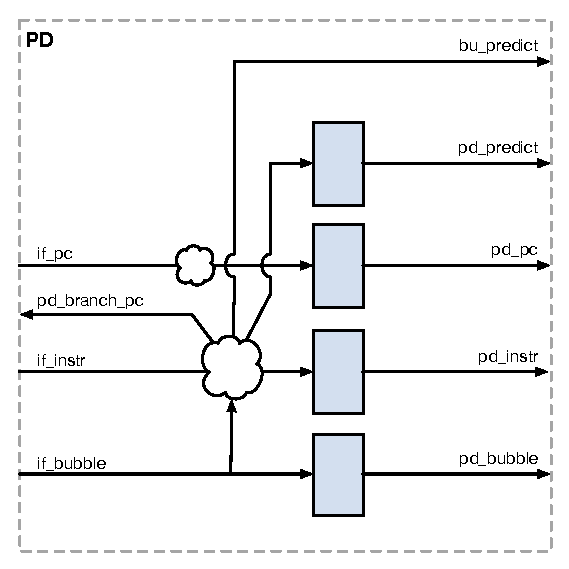
\includegraphics{assets/img/Pipeline-PD}
  \caption{Instruction Pre-Decode Stage}
\end{figure}

\begin{longtable}[]{@{}lccl@{}}
	\toprule
	\textbf{Signal} & \textbf{Direction} & \textbf{To/From} & \textbf{Description}\tabularnewline
	\midrule

\ifdefined\MARKDOWN
	\endhead
\else
	\endfirsthead
	\multicolumn{4}{c}{{(Continued from previous page)}} \\
	\toprule
	\textbf{Signal} & \textbf{Direction} & \textbf{To/From} & \textbf{Description}\tabularnewline
	\midrule
	\endhead
	\midrule \multicolumn{4}{c}{{\tablename\ \thetable{} continued on next page\ldots}} \\
	\endfoot
	\endlastfoot

\fi

	\texttt{if\_pc}         & from & IF & Instruction Fetch program counter\\
	\texttt{if\_instr}      & from & IF & Instruction Fetch instruction\\
	\texttt{if\_bubble}     & from & IF & Instruction Fetch bubble\\
	\texttt{if\_exception}  & from & IF & Instruction Fetch exception status\\
	\texttt{pd\_branch\_pc} & to   & IF & New PC (for a branch instruction)\\
	& & &\\
	\texttt{bu\_predict}    & from & BP & Branch prediction from Branch Prediction Unit\\
	\texttt{pd\_predict }   & to   & ID & Forwarded branch prediction\\
	\texttt{pd\_pc}         & to   & ID & Pre-Decode program counter\\
	\texttt{pd\_instr}      & to   & ID & Pre-Decode instruction\\
	\texttt{pd\_bubble}     & to   & ID & Pre-Decode bubble\\
	\texttt{pd\_exception}  & to   & ID & Pre-Decode exception status\\
	\bottomrule
	\caption{PD Signals}
	\label{tab:pd-signals}
\end{longtable}

\pagebreak

\section{Instruction Decode (ID)}\label{instruction-decode-id-1}

The Instruction Decode unit ensures the operands for the execution units are available.
It accesses the Register File, calculates immediate values, sets bypasses, and checks for illegal opcodes and opcode combinations.

\begin{figure}[h]
  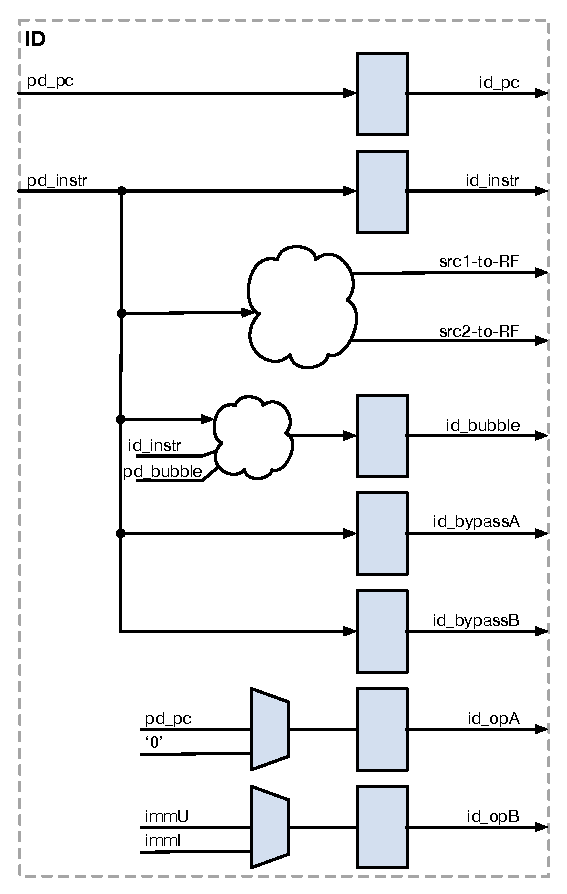
\includegraphics{assets/img/Pipeline-ID}
  \caption{Instruction Decode Stage Implementation}
\end{figure}

\begin{longtable}[]{@{}lccl@{}}
	\toprule
	\textbf{Signal} & \textbf{Direction} & \textbf{To/From} & \textbf{Description}\tabularnewline
	\midrule

\ifdefined\MARKDOWN
	\endhead
\else
	\endfirsthead
	\multicolumn{4}{c}{{(Continued from previous page)}} \\
	\toprule
	\textbf{Signal} & \textbf{Direction} & \textbf{To/From} & \textbf{Description}\tabularnewline
	\midrule
	\endhead
	\midrule \multicolumn{4}{c}{{\tablename\ \thetable{} continued on next page\ldots}} \\
	\endfoot
	\endlastfoot
\fi

		\texttt{pd\_pc}	       & from & PD & Pre-Decode program counter\\
		\texttt{pd\_instr}     & from & PD & Pre-Decode instruction\\
		\texttt{pd\_bubble}    & from & PD & Pre-Decode bubble\\
		\texttt{pd\_exception} & from & PD & Pre-Decode exception status\\
		& & &\\
		\texttt{src1}          & to   & RF & Source Register1 index\\
		\texttt{src2}          & to   & RF & Source Register2 Index\\
		& & &\\
		\texttt{id\_bypassA}   & to   & EX & Bypass signals for srcA\\
		\texttt{id\_bypassB}   & to   & EX & Bypass signals for srcB\\
		\texttt{id\_opA}       & to   & EX & Calculated operandA\\
		\texttt{id\_opB}       & to   & EX & Calculated operandB\\
		\texttt{id\_pc}        & to   & EX & Instruction Decode program counter\\
		\texttt{id\_instr}     & to   & EX & Instruction Decode instruction\\
		\texttt{id\_bubble}    & to   & EX & Instruction Decode bubble\\
		\texttt{id\_exception} & to   & EX & Instruction Decode exception status\\
	\bottomrule
	\caption{ID Signals}
	\label{tab:id-signals}
\end{longtable}

\pagebreak

\section{Execute (EX)}\label{execute-ex-1}

The Execute stage performs the required operation on the data provided by the Instruction Decode stage.
The Execution stage has multiple execution units, each with a unique function.
The ALU performs logical and arithmetic operations.
The Multiplier unit calculates signed/unsigned multiplications.
The Divider unit calculates signed/unsigned division and remainder.
The Load-Store Unit accesses the data memory.
The Branch Unit calculates jump and branch addresses and validates the predicted branches.

Only one operation can be executed per clock cycle.
Most operations complete in one clock cycle, except for the divide instructions, which always take multiple clock cycles to complete.
The multiplier supports configurable latencies, to improve performance.


\begin{figure}[h]
  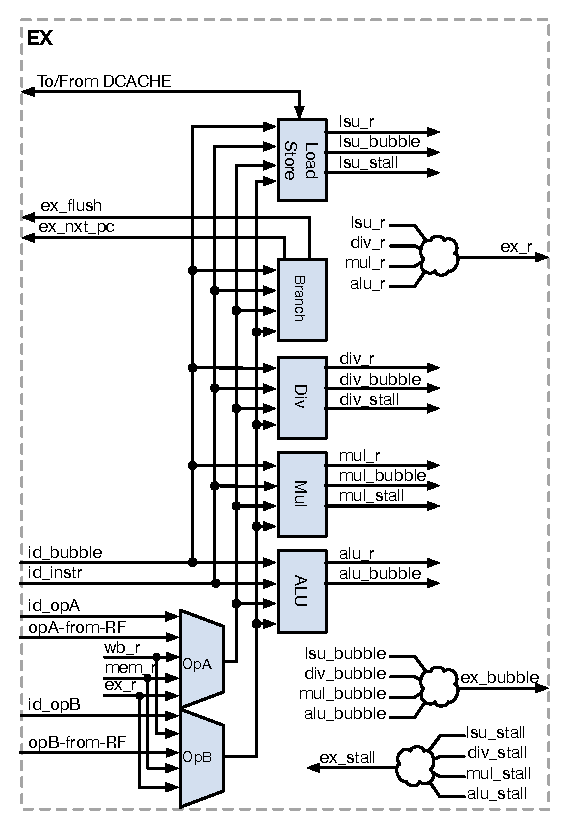
\includegraphics{assets/img/Pipeline-EX}
  \caption{Execute Stage Implementation}
\end{figure}

\begin{longtable}[]{@{}lccl@{}}
	\toprule
	\textbf{Signal} & \textbf{Direction} & \textbf{To/From} & \textbf{Description}\tabularnewline
	\midrule

\ifdefined\MARKDOWN
	\endhead
\else
	\endfirsthead
	\multicolumn{4}{c}{{(Continued from previous page)}} \\
	\toprule
	\textbf{Signal} & \textbf{Direction} & \textbf{To/From} & \textbf{Description}\tabularnewline
	\midrule
	\endhead
	\midrule \multicolumn{4}{c}{{\tablename\ \thetable{} continued on next page\ldots}} \\
	\endfoot
	\endlastfoot
\fi
		\texttt{id\_pc}        & from & ID       & Instruction Decode program counter\\
		\texttt{id\_instr}     & from & ID       & Instruction Decode instruction\\
		\texttt{id\_bubble}    & from & ID       & Instruction Decode bubble\\
		\texttt{id\_exception} & from & ID       & Instruction Decode exception status\\
		                       &      &          & \\
		\texttt{opA}           & from & RF       & Source Register1 value\\
		\texttt{opB}           & from & RF       & Source Register2 value\\
		                       &      &          & \\
		\texttt{id\_bypassA}   & from & ID       & Bypass signals for srcA\\
		\texttt{id\_bypassB}   & from & ID       & Bypass signals for srcB\\
		\texttt{id\_opA}       & from & ID       & Calculated operandA\\
		\texttt{id\_opB}       & from & ID       & Calculated operandB\\
		\texttt{ex\_stall}     & to   & ID       & Stall ID (and higher) stages\\
		\texttt{ex\_flush}     & to   & ID/PD/IF & Flush ID (and higher) pipe stages\\
		\texttt{ex\_r}         & to   & MEM      & Result from execution units\\
		\texttt{ex\_pc}        & to   & MEM      & Execute program counter\\
		\texttt{ex\_instr}     & to   & MEM      & Execute instruction\\
		\texttt{ex\_bubble}    & to   & MEM      & Execute bubble\\
		\texttt{ex\_exception} & to   & MEM      & Execute exception status\\
	\bottomrule
	\caption{EX Signals}
	\label{tab:ex-signals}
\end{longtable}

\pagebreak


\section{Memory-Access (MEM)}\label{memory-access-mem-1}

The Memory Access stage waits for a memory read access to complete.
When memory is accessed, address, data, and control signals are calculated during the Execute stage.
The memory latches these signals and then performs the actual access. This means that read-data won't be available until 1 clock cycle later.
This would be at the end of the Write-Back stage, and hence too late. Therefore the Memory-Access stage is added.

\begin{figure}[h]
  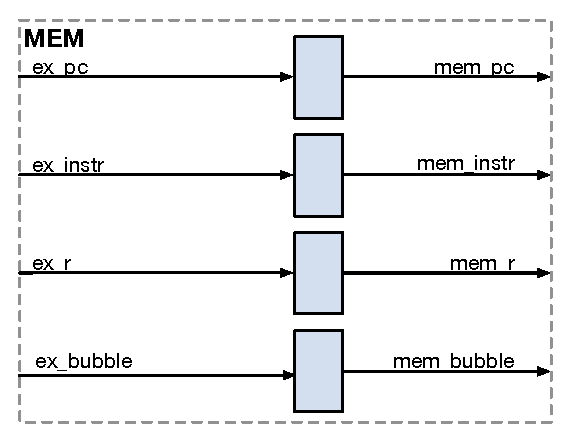
\includegraphics{assets/img/Pipeline-MEM}
  \caption{Memory Stage Implementation}
\end{figure}

\begin{longtable}[]{@{}lccl@{}}
	\toprule
	\textbf{Signal} & \textbf{Direction} & \textbf{To/From} & \textbf{Description}\tabularnewline
	\midrule
\ifdefined\MARKDOWN
	\endhead
\else
	\endfirsthead
	\multicolumn{4}{c}{{(Continued from previous page)}} \\
	\toprule
	\textbf{Signal} & \textbf{Direction} & \textbf{To/From} & \textbf{Description}\tabularnewline
	\midrule
	\endhead
	\midrule \multicolumn{4}{c}{{\tablename\ \thetable{} continued on next page\ldots}} \\
	\endfoot
	\endlastfoot
\fi
		\texttt{ex\_r}          & from & EX       & Result from Execution stage\\
		\texttt{ex\_pc}         & from & EX       & Execute program counter\\
		\texttt{ex\_instr}      & from & EX       & Execute instruction\\
		\texttt{ex\_bubble}     & from & EX       & Execute bubble\\
		\texttt{ex\_exception}  & from & EX       & Execute stage exception status\\
		                        &      &          & \\
		\texttt{mem\_r}         & to   & WB/EX    & Memory Access result\\
		\texttt{mem\_instr}     & to   & WB/ID    & Memory Access instruction\\
		\texttt{mem\_bubble}    & to   & WB/ID    & Memory Access bubble\\
		\texttt{mem\_exception} & to   & WB/ID/EX & Memory Access exception status\\

	\bottomrule
	\caption{MEM Signals}
	\label{tab:mem-signals}
\end{longtable}

\pagebreak


\section{Write-Back (WB)}\label{write-back-wb-1}

The Write-Back stage writes the results from the Execution Units and memory-read operations into the Register File.

\begin{figure}[h]
  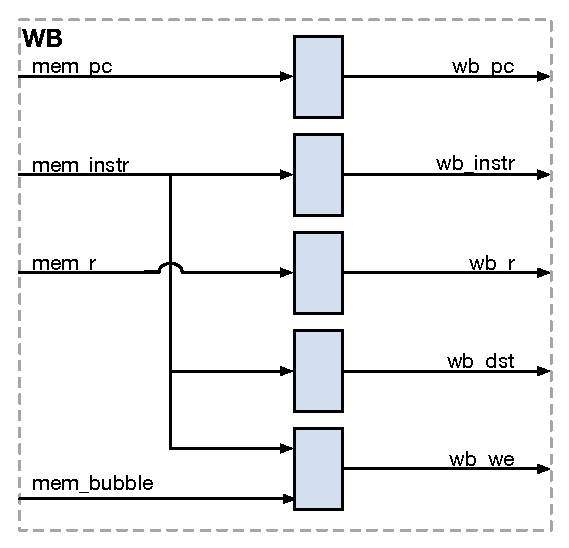
\includegraphics{assets/img/Pipeline-WB}
  \caption{Write-back Stage Implementation}
\end{figure}

\begin{longtable}[]{@{}lccl@{}}
	\toprule
	\textbf{Signal} & \textbf{Direction} & \textbf{To/From} & \textbf{Description}\tabularnewline
	\midrule
\ifdefined\MARKDOWN
	\endhead
\else
	\endfirsthead
	\multicolumn{4}{c}{{(Continued from previous page)}} \\
	\toprule
	\textbf{Signal} & \textbf{Direction} & \textbf{To/From} & \textbf{Description}\tabularnewline
	\midrule
	\endhead
	\midrule \multicolumn{4}{c}{{\tablename\ \thetable{} continued on next page\ldots}} \\
	\endfoot
	\endlastfoot
\fi
		\texttt{mem\_r}         & from & MEM         & Result from Memory Access stage\\
		\texttt{mem\_pc}        & from & MEM         & Memory Access program counter\\
		\texttt{mem\_instr}     & from & MEM         & Memory Access instruction\\
		\texttt{mem\_exception} & from & MEM         & Memory Access exception status\\\
		\texttt{mem\_bubble}    & from & MEM         & Memory Access bubble\\
		\texttt{dmem\_q}        & from & Data Memory & Result from Data Memory\\
		\texttt{dmem\_ack}      & from & Data Memory & Data Memory acknowledge\\
		                        &      &             & \\
		\texttt{wb\_r}          & to   & RF/ID/EX    & Result to be written to RF\\
		\texttt{wb\_dst}        & to   & RF          & Destination register index\\
		\texttt{wb\_we}         & to   & RF          & Write enable\\
		\texttt{wb\_pc}         & to   & State       & WriteBack program counter\\
		\texttt{wb\_instr}      & to   & State/ID    & WriteBack instruction\\
		\texttt{wb\_bubble}     & to   & State/ID    & WriteBack bubble\\
		\texttt{wb\_exception}  & to   & State/ID/EX & WriteBack exception status\\

	\bottomrule
	\caption{WB Signals}
	\label{tab:wb-signals}
\end{longtable}


